\documentclass[a4paper,landscape]{article}

%%{ packages

\usepackage[landscape]{geometry}
\usepackage{url}
\usepackage{multicol}
\usepackage{amsmath}
\usepackage{amsfonts}
\usepackage{tikz}
\usepackage{amsmath,amssymb}
\usepackage{colortbl}
\usepackage{xcolor}
\usepackage{mathtools}
\usepackage{amsmath,amssymb}
\usepackage{listings}
\usepackage{pdfpages}
\lstset{
  basicstyle=\ttfamily,
  frame=single
  }
  \usepackage{enumitem}
  \usepackage[english]{babel}
  \usepackage[utf8]{inputenc}
  \usetikzlibrary{decorations.pathmorphing}

  %%}

  \title{MRS lab ROS platform Cheat Sheet}

  \advance\topmargin-.8in
  \advance\textheight3in
  \advance\textwidth3in
  \advance\oddsidemargin-1.5in
  \advance\evensidemargin-1.5in
  \parindent0pt
  \parskip2pt

  \newcommand{\hr}{\centerline{\rule{3.5in}{1pt}}}

  %\colorbox[HTML]{e4e4e4}{\makebox[\textwidth-2\fboxsep][l]{texto}

  \begin{document}

  \begin{center}{\huge{\textbf{MRS lab ROS platform Cheat Sheet}}}\\
    {\large by Tomas Baca @ Multi-robot Systems (MRS), v1.2.0}
  \end{center}

  \begin{multicols*}{2}

    \tikzstyle{mybox} = [draw=black, fill=white, very thick,
    rectangle, rounded corners, inner sep=10pt, inner ysep=10pt]
    \tikzstyle{fancytitle} =[fill=black, text=white, font=\bfseries]

    %%{ TERMINAL BASICS

    \begin{tikzpicture}
      \node [mybox] (box){%
        \begin{minipage}{0.47\textwidth}
          \begin{center}
            \scriptsize{
              \textbf{Hitting $\langle\mathrm{Tab}\rangle$ autocompletes commands, filenames, etc.}
              \begin{tabular}{lp{6.0cm} r}
                \hline
                New terminal & \texttt{Ctrl+Alt+t} \\ \hline
                \textbf{Need help} & append \texttt{--help} after command\\
                \textbf{Need more help!} & \texttt{:\$ man [command]} \\ \hline
                Change directory & \texttt{:\$ cd [path]} \\ \hline
                Path symbolic links & $\texttt{.}$ -- current directory \\
                & $\texttt{..}$ -- previous directory \\
                & $\texttt{$\sim$}$ -- home directory (also \texttt{\$HOME})\\
                & $\texttt{/}$ -- root directory \\ \hline
                create a file & \texttt{:\$ touch [path]} \\
                remove a file & \texttt{:\$ rm [path]} \\
                move (also rename) a file & \texttt{:\$ mv [from] [to]} \\
                copy a file & \texttt{:\$ cp [from] [to]} \\
                print a file & \texttt{:\$ cat [path]} \\
                edit a file & \texttt{:\$ vim [path]}, \texttt{:\$ nano [path]} \\ \hline
                set a variable & \texttt{:\$ VARIABLE="dog", VARIABLE=3.0} \\
                print a variable & \texttt{:\$ echo "the content is: \$VARIABLE"} \\ \hline
                run a script or executable& \texttt{:\$ ./script.sh, ./program} \\ \hline
                output redirection & $\texttt{>}$ -- to a file (rewrite) \\
                & $\texttt{>>}$ -- to a file (append) \\
                & $\texttt{|}$ -- pipe to another command \\
                redirect to /dev/null & $\texttt{> /dev/null 2>\&1}$ \\ \hline
              \end{tabular}
            }

            \vspace{0.2em}
            Would You Like to Know More? \url{http://google.com}
            \vspace{-1em}
          \end{center}
        \end{minipage}
        };
        \node[fancytitle, right=10pt] at (box.north west) {Ubuntu terminal - GNU/Linux basics};
    \end{tikzpicture}

    %%}

    %%{ TMUX

    \begin{tikzpicture}
      \node [mybox] (box){%
        \begin{minipage}{0.47\textwidth}
          \begin{center}
            \scriptsize{
              \begin{tabular}{lp{4.0cm} r}
                \hline
                Run tmux & \texttt{:\$ tmux} \\
                List all sessions & \texttt{:\$ tmux ls} \\
                Attach to a session & \texttt{:\$ tmux a -t [session name]} \\
                \hline
                New window (tab) & \texttt{Ctrl+t}\\
                New horizontal split & \texttt{Ctrl+9}\\
                New vertical split & \texttt{Ctrl+0}\\
                Moving through windows (tabs) & \texttt{Shift+$\rightarrow$}, \texttt{Shift+$\leftarrow$}  \\
                Moving through panes (splits) & \texttt{Alt+$\rightarrow$}, \texttt{Alt+$\leftarrow$}, \texttt{Alt+$\uparrow$}, \texttt{Alt+$\downarrow$} \\
                \hline
                \textbf{prefix} & \texttt{Ctrl+a}\\
                \hline
                Killing window & \textbf{prefix} \texttt{x}, \texttt{:\$ exit}, \texttt{:\$ :q}\\
                Killing session & \textbf{prefix} \texttt{k}\\
                Detach from session & \textbf{prefix} \texttt{d}\\
                Enter vim mode (scrolling, copying) & \texttt{F2}, \textbf{prefix} \texttt{$[$}\\
                \hline
              \end{tabular}
            }

            \vspace{0.2em}
            Would You Like to Know More? \url{https://github.com/klaxalk/linux-setup/wiki/tmux}
            \vspace{-1em}
          \end{center}
        \end{minipage}
        };
        \node[fancytitle, right=10pt] at (box.north west) {TMUX - Terminal multiplexer};
    \end{tikzpicture}

    %%}

    %%{ VIM

    \begin{tikzpicture}
      \node [mybox] (box){%
        \begin{minipage}{0.47\textwidth}
          \scriptsize{
            Vim is not a joke. Although you might not know how to exit it (yet), it is a very powerful tool.
            Our vim is filled with features, including code snippets, code completion (ROS aware), code formatting, syntax highlighting and tmux integration.
            Its control is completely mouse-less and it is fully usable over ssh, which makes it great for remote editing on a drone.
            Moreover, its modal editing paradigm is very intuitive.
            Lastly, when you learn how to control vim, you also learn to control other tools such as \emph{Linux manual pages}, \emph{ranger}, \emph{less} and much more.
            Even gmail uses vim-like controls natively.
            Run \texttt{:\$ vimtutor} to start learning vim using an interactive ``file tutorial''.
            Here are some simple commands:
            \begin{center}
              \begin{tabular}{lp{1cm} r lp{1cm} r}
                \hline
                switch to insert mode & \texttt{i} & jump a word/Word forwards & \texttt{w}/\texttt{W} \\
                return to normal mode & \texttt{ESC} & jump a word/Word backwards & \texttt{b}/\texttt{B} \\
                cut a line to clipboard & \texttt{dd} & change current word/Word & \texttt{ciw}/\texttt{ciW} \\
                paste a clipboard & \texttt{p} & delete 3 lines down & \texttt{3dj} \\
                \hline
                open a command line & \texttt{:} & substitute \emph{dog} for \emph{cat} & \texttt{:\%s/dog/cat/g} \\
                save & \texttt{:w} & move cursor left/down/up/right & h/j/k/l\\
                quit & \texttt{:q} & delete every line containing \emph{dog} & \texttt{:\%g/dog/normal dd} \\
                \hline
              \end{tabular}

              \vspace{0.2em}
              Would You Like to Know More? \url{https://www.tutorialspoint.com/vim/}
              \vspace{-1em}
            \end{center}
            }
        \end{minipage}
        };
        \node[fancytitle, right=10pt] at (box.north west) {Vim -- a modern modular text processor};
    \end{tikzpicture}

    %%}

    %%{ GIT

    \begin{tikzpicture}
      \node [mybox] (box){%
        \begin{minipage}{0.47\textwidth}
          \scriptsize{Git is a distributed version control system.
          Repositories are equal, some are just used as a ``server'' (called \textbf{remote}).
          Git uses branches to isolate ongoing work on the same project.
          Branches can be merged to combine the work back into a single piece.
          Changes in the files should be \textbf{commited}.
          Only commit ``runnable'' code.}
          \begin{center}
            \scriptsize{
              \begin{tabular}{lp{8.0cm} r}
                \hline
                Cloning a repository & over ssh \texttt{:\$ git clone git@mrs.felk.cvut.cz:uav/uav\_core} \\
                & over https \texttt{:\$ git clone https://github.com/klaxalk/linux-setup} \\
                \hline
                Update origin state & \texttt{:\$ git fetch} \\
                Update current branch from remote & \texttt{:\$ git pull} \\
                Update current branch to remote & \texttt{:\$ git push} \\
                Commit ``patch'' -- interactive  & \texttt{:\$ git commit -p} \\
                Add files for commit & \texttt{:\$ git add [file]} \\
                Commit changes & \texttt{:\$ git commit -m "commit message"} \\
                \hline
                Checkout a branch & \texttt{:\$ git checkout [branch name]} \\
                Create a branch & \texttt{:\$ git checkout -b [branch name]} \\
                \hline
                unstage the file & \texttt{:\$ git reset [file name]} \\
                undo all uncommited changes & \texttt{:\$ git reset --hard} \\
                remove all new unstaged files & \texttt{:\$ git clean -fd} \\
                \hline
                Merge a branch & \texttt{:\$ git merge [branch name]} \\
                Rebase on a branch & \texttt{:\$ git rebase [branch name]} \\
                \hline
                refactor branch history & \texttt{:\$ git filter-branch [lot of args]} \\
                \hline
                show status & \texttt{:\$ git status} \\
                show log & \texttt{:\$ git log} \\
                show better log & \texttt{:\$ glog} \\
                % & -- is an alias for \texttt{:\$ git log --graph --abbrev-commit --date=relative --pretty=format:'\%Cred\%h\%Creset -\%C(yellow)\%d\%Creset \%s \%Cgreen(\%cr) \%C(bold blue)<\%an>\%Creset'} \\
                & -- is an alias for \texttt{:\$ git log} with more arguments\\
                show super forest log & \texttt{:\$ flog} \\
                & -- uses \texttt{~/.scripts/git-forest.sh} \\
                \hline
              \end{tabular}

              \vspace{0.2em}
              Would You Like to Know More? \url{https://try.github.io/}
              \vspace{-1em}
            }
          \end{center}
        \end{minipage}
        };
        \node[fancytitle, right=10pt] at (box.north west) {Git version control system};
    \end{tikzpicture}

    %%}

    %%{ .bashrc

    \begin{tikzpicture}
      \node [mybox] (box){%
        \begin{minipage}{0.47\textwidth}
          \scriptsize{
            When a new terminal is opened and an instance of bash is launched, the \texttt{$\sim$/.bashrc} file is \emph{sourced} (executed while its leftover variables, functions and aliases stay in the context).
            We use \texttt{.bashrc} heavily for setting context for ROS and our development environment.
            \texttt{.bashrc} sources ROS setup scripts, which are also generated by each workspace.
            If you change this file, source it (or open a new terminal) to activate the changes: \texttt{:\$ source $\sim$/.bashrc} or just \texttt{:\$ sb}.
            Here is an example of what should not be missing in the bottom of a healthy \texttt{.bashrc} file:
            \vspace{-1.5em}
            \begin{center}
              \begin{lstlisting}
        source /opt/ros/melodic/setup.bash
        source /usr/share/gazebo/setup.sh

        source ~/workspace/devel/setup.bash
        # source ~/other_workspace/devel/setup.bash

        export ROS_WORKSPACES="~/mrs_workspace ~/workspace"

        export GIT_PATH=$HOME/git

        export RUN_TMUX=true

        # VARIABLES TO CONFIGURE THE MRS ROS PIPELINE
        export UAV_NAME="uav1"
        ...
        export MRS_STATUS="readme"

        source $GIT_PATH/uav_core/miscellaneous/shell_additions/shell_additions.sh

        source $GIT_PATH/linux-setup/appconfig/bash/dotbashrc
              \end{lstlisting}
              \vspace{-1.5em}
            \end{center}
          }
        \end{minipage}

        };
        \node[fancytitle, right=10pt] at (box.north west) {.bashrc -- Bash configuration};
    \end{tikzpicture}

    %%}

    %%{ ROS IN LINUX TERMINAL

    \begin{tikzpicture}
      \node [mybox] (box){%
        \begin{minipage}{0.47\textwidth}
          \begin{center}
            \scriptsize{
              \textbf{Please}, visit \url{http://wiki.ros.org/ROS/Tutorials} before starting work on a bigger project.\\
              \textbf{Use $\langle\mathrm{Tab}\rangle$ to complete commands, topic names, message types and pre-fill message contents.}

              \begin{tabular}{lp{6.0cm} r}
                \hline
                Getting help & append \texttt{--help} after any following command\\
                \hline
                Listing all ROS nodes & \texttt{:\$ rosnode list} \\
                Listing all ROS topics & \texttt{:\$ rostopic list} \\
                Listing all ROS services & \texttt{:\$ rosservice list} \\
                Listing all ROS params & \texttt{:\$ rosparam list} \\
                \hline
                Running a ROS binary & \texttt{:\$ rosrun package\_name binary\_name} \\
                Running a launch file & \texttt{:\$ roslaunch package\_name launch\_file.launch} \\
                \hline
                Showing a node info & \texttt{:\$ rosnode info /node/path} \\
                Showing a topic info & \texttt{:\$ rostopic info /topic/path} \\
                Showing a service info & \texttt{:\$ rosservice info /service/path} \\
                \hline
                Showing a topic type & \texttt{:\$ rostopic type /topic/path} \\
                Showing a service type & \texttt{:\$ rosservice type /topic/path} \\
                \hline
                Showing a message type structure & \texttt{:\$ rosmsg show [msg type]} \\
                Showing a service type structure & \texttt{:\$ rossrv show [srv type]} \\
                \hline
                Showing topic messages & \texttt{:\$ rostopic echo /topic/path} \\
                Showing a param value & \texttt{:\$ rosparam get /parm/path} \\
                \hline
                Calling a service & \texttt{:\$ rosservice call /service/path [args]} \\
                Publishing on a topic & \texttt{:\$ rostopic pub /topic/path [args]} \\
                Setting a param value & \texttt{:\$ rosparam set /parm/path [args]} \\
                \hline
              \end{tabular}
            }

            \vspace{0.2em}
            Would You Like to Know More? \url{http://wiki.ros.org/ROS/CommandLineTools}
            \vspace{-1em}
          \end{center}
        \end{minipage}
        };
        \node[fancytitle, right=10pt] at (box.north west) {ROS in Linux terminal};
    \end{tikzpicture}

    %%}

    %%{ ROS WORKSPACE STRUCTURE

    \begin{tikzpicture}
      \node [mybox] (box){%
        \begin{minipage}{0.47\textwidth}
          \subsubsection*{MRS lab main workspace}
          \begin{center}
            \scriptsize{
              \begin{tabular}{lp{6.0cm} r}
                \hline
                path & \texttt{$\sim$/mrs\_workspace/}\\
                contains & \texttt{src/uav\_core/} -- core MRS repository\\
                & \texttt{src/uav\_modules/} -- modules MRS repository\\
                \hline
              \end{tabular}
            }
          \end{center}
          \subsubsection*{MRS lab student workspace}
          \begin{center}
            \scriptsize{
              \begin{tabular}{lp{6.0cm} r}
                \hline
                path & \texttt{$\sim$/workspace}\\
                contains & \texttt{example\_packages/}\\
                & -- \texttt{waypoint\_flier} -- general example\\
                & -- \texttt{vision\_example} -- computer vision template\\
                \hline
              \end{tabular}
            }
          \end{center}
          \subsubsection*{General ROS package structure}
          \begin{center}
            \scriptsize{
              \begin{tabular}{lp{8.0cm} r}
                \hline
                \texttt{build} & generated makefiles and support files\\
                & \textbf{do not modify}\\
                \texttt{devel} & compiled binaries, libraries and installed headers\\
                & \textbf{do not modify}\\
                \texttt{src} & package source codes\\
                & \textbf{place your stuff in here}\\
                \hline
              \end{tabular}
            }

            \scriptsize{
              \vspace{0.2em}
              \vspace{-1em}
            }
          \end{center}
        \end{minipage}
        };
        \node[fancytitle, right=10pt] at (box.north west) {ROS workspace structure};
    \end{tikzpicture}

    %%}

    %%{ NAVIGATING AND COMPILING ROS WORKSPACE

    \begin{tikzpicture}
      \node [mybox] (box){%
        \begin{minipage}{0.47\textwidth}
          \begin{center}
            \scriptsize{
              \begin{tabular}{lp{5cm} r}
                \hline
                go to a package & \texttt{:\$ roscd [package name]}\\
                \hline
                compile the whole workspace & \texttt{:\$ catkin build}\\
                compile a particular package & \texttt{:\$ catkin build [package name]}\\
                compile current package & \texttt{:\$ catkin bt}\\
                clean the whole workspace & \texttt{:\$ catkin clean}\\
                clean a particular package & \texttt{:\$ catkin clean [package name]}\\
                \hline
                show workspace config & \texttt{:\$ catkin config}\\
                show compilation profiles & \texttt{:\$ catkin profile list}\\
                set a compilation profile & \texttt{:\$ catkin profile set [profile name]}\\
                \hline
                create a new workspace & \texttt{:\$ catkin init}\\
                set workspace extending & \texttt{:\$ catkin config --extend [path]}\\
                \hline
              \end{tabular}

              \vspace{0.2em}
              Would You Like to Know More? \url{https://catkin-tools.readthedocs.io/en/latest/}
              \vspace{-1em}
            }
          \end{center}
        \end{minipage}
        };
        \node[fancytitle, right=10pt] at (box.north west) {Navigating and compiling ROS workspace};
    \end{tikzpicture}

    %%}

    %%{ ROS PACKAGE STRUCTURE

    \begin{tikzpicture}
      \node [mybox] (box){%
        \begin{minipage}{0.47\textwidth}
          \scriptsize {Some of the following items might be missing, depending on the package use case.}
          \begin{center}
            \scriptsize{
              \begin{tabular}{lp{5.5cm} r}
                \hline
                \texttt{package.xml} & manifest, dependencies and plugins\\
                \texttt{CMakeLists.txt} & description of compilation procedure\\
                \texttt{src/} & \verb!C! and \verb!C++! source codes\\
                \texttt{include/} & \verb!C! and \verb!C++! headers\\
                \texttt{scripts/} & Python and bash scripts\\
                \texttt{config/} & yaml config files\\
                \texttt{cfg/} & dynamic reconfigure scripts\\
                \texttt{launch/} & ROS launch files\\
                \hline
              \end{tabular}
            }

            \vspace{0.2em}
            Would You Like to Know More? \url{http://wiki.ros.org/Packages}
            \vspace{-1em}
          \end{center}
        \end{minipage}
        };
        \node[fancytitle, right=10pt] at (box.north west) {ROS package structure};
    \end{tikzpicture}

    %%}

    %%{ ROS VISUALIZATION TOOLS

    \begin{tikzpicture}
      \node [mybox] (box){%
        \begin{minipage}{0.47\textwidth}
          \begin{center}
            \scriptsize{
              \begin{tabular}{lp{6cm} r}
                \hline
                Rviz & 3-D visualization of data and models \\
                & \texttt{:\$ rviz} \\
                & \texttt{:\$ roslaunch mrs\_testing rviz\_uav1.launch} \\ \hline
                Rqt plot & simple and lightweight plotting \\
                & \texttt{:\$ rqt\_plot} \\ \hline
                Rqt bag & visualizing contents of a rosbag \\
                & \texttt{:\$ rqt\_bag} \\ \hline
                Plot juggler & complex and powerful plotting \\
                & \texttt{:\$ rosrun plotjuggler PlotJuggler} \\ \hline
                Rqt reconfigure & online parameter setting \\
                & \texttt{:\$ rosrun rqt\_reconfigure rqt\_reconfigure} \\ \hline
                Rqt image view & camera images visualization \\
                & \texttt{:\$ rqt\_image\_view} \\ \hline
                Gazebo client & Gazebo GUI \\
                & \texttt{:\$ gzclient} \\ \hline
                rqt & Integrates most of the \textit{rqt\_} tools \\
                & \texttt{:\$ rqt} \\ \hline
              \end{tabular}
            }

            \vspace{0.2em}
            Would You Like to Know More? \url{http://wiki.ros.org/Tools}
            \vspace{-1em}
          \end{center}
        \end{minipage}
        };
        \node[fancytitle, right=10pt] at (box.north west) {ROS visualization tools};
    \end{tikzpicture}

    %%}

    %%{ USEFUL UAV ROS TOPICS AND SERVICES

    \begin{tikzpicture}
      \node [mybox] (box){%
        \begin{minipage}{0.47\textwidth}
          \scriptsize{
            Following ROS services and topics allow for controlling the UAV from terminal.
            Each address contains a particular name of the UAV.
          }
          \subsubsection*{Informative topics (subscribe to know stuff)}
          \begin{center}
            \scriptsize{
              \begin{tabular}{lp{6cm} r}
                \hline
                state estimate (rviz-able) & \texttt{/uav1/odometry/odom\_main}\\
                control reference (rviz-able) & \texttt{/uav1/control\_manager/cmd\_odom}\\
                control reference (full-state) & \texttt{/uav1/control\_manager/position\_cmd}\\
                control manager diagnostics & \texttt{/uav1/control\_manager/diagnostics}\\
                \hline
              \end{tabular}
            }
          \end{center}
          \subsubsection*{Control Services/Topics (call or publish to influence stuff)}
          \begin{center}
            \scriptsize{
              The addresses for \emph{reference}, \emph{trajectory\_reference} are the same for both the topic and the service.
              \vspace{0.2em}
              \begin{tabular}{lp{8cm} r}
                \hline
                position+heading goal & \texttt{/uav1/control\_manager/reference}\\
                \hline
                takeoff & \texttt{/uav1/uav\_manager/takeoff}\\
                land & \texttt{/uav1/uav\_manager/land}\\
                land home & \texttt{/uav1/uav\_manager/land\_home}\\
                hover & \texttt{/uav1/uav\_manager/hover}\\
                \hline
                switch controller & \texttt{/uav1/control\_manager/switch\_controller [Controller]}\\
                switch tracker & \texttt{/uav1/control\_manager/switch\_tracker [Tracker]}\\
                set tracker constraints & \texttt{/uav1/constraint\_manager/set\_constraints [Constraints]}\\
                set SO(3) controller gains & \texttt{/uav1/gain\_manager/set\_gains [Gains]}\\
                \hline
                load trajectory & \texttt{/uav1/control\_manager/trajectory\_reference}\\
                trajectory goto start & \texttt{/uav1/control\_manager/goto\_trajectory\_start}\\
                trajectory start tracking & \texttt{/uav1/control\_manager/start\_trajectory\_tracking}\\
                \hline
              \end{tabular}

              \vspace{0.2em}
              \tiny Would You Like to Know More? \url{https://ctu-mrs.github.io/docs/system/uav_ros_interface.html}
              \vspace{-1em}
            }
          \end{center}
        \end{minipage}
        };
        \node[fancytitle, right=10pt] at (box.north west) {Useful UAV ROS topics and services};
    \end{tikzpicture}

    %%}

    \clearpage

    %%{ SSH keys

    \begin{tikzpicture}
      \node [mybox] (box){%
        \begin{minipage}{0.47\textwidth}
          \scriptsize{
            \begin{itemize}
              \setlength\itemsep{0.0em}
              \item Generate your SSH key by: \texttt{:\$ ssh-keygen -t rsa -b 4096 -C "your\_email@example.com"}.
              \item The keys are stored in \texttt{$\sim$/.ssh}.
              \item Show the content of the public key by: \texttt{:\$ cat $\sim$/.ssh/id\_rsa.pub} and copy it to Github or Gitlab.
              \item Copy your public key over ssh to another machine by: \texttt{:\$ ssh-copy-id user@machine}.
              \item Entries in the \texttt{$\sim$/.ssh/config} allow connecting to a machine via alias while using an ssh key:
            \end{itemize}
            \vspace{-2.8em}
            \begin{center}
              \begin{lstlisting}
                        host mrs
                             hostname mrs.felk.cvut.cz
                             user git
                             identityfile ~/.ssh/id_rsa
              \end{lstlisting}
            \end{center}
            \vspace{-3.0em}
          }
        \end{minipage}
        };
        \node[fancytitle, right=10pt] at (box.north west) {SSH keys};
    \end{tikzpicture}

    %%}

    %%{ UAV SPAWNING

    \begin{tikzpicture}
      \node [mybox] (box){%
        \begin{minipage}{0.47\textwidth}
          \scriptsize{
            We use a ROS node called \texttt{mrs\_drone\_spawner} to dynamically load a UAV into the Gazebo/ROS simulator.
            By default, it starts automatically with Gazebo using \texttt{:\$ roslaunch mrs\_simulation simulation.launch}. \\
            Spawn a drone by calling a service \texttt{:\$ rosservice call /mrs\_drone\_spawner/spawn "1 --enable-rangefinder"} \\
            If the service does not exist, start the spawner by \texttt{:\$ roslaunch mrs\_simulation mrs\_drone\_spawner.launch} \\
            Various arguments can be used to influence the type of the drone, its sensors, its starting location and additional onboard hardware.
            Run the command \texttt{:\$ rosrun mrs\_simulation mrs\_drone\_spawner.py} to see the complete list. Here are some notable examples:
            \begin{center}
              \begin{tabular}{lp{5cm} r}
                \hline
                use initial position from a CSV file (id, x, y, z, heading) & \texttt{--file [path\_to\_file]} \\
                use initial position from an argument & \texttt{--pos [x y z heading]} \\
                selecting UAV type (f450, f550, t650) & \texttt{--f450}, \texttt{--f550}, \texttt{--t650} \\
                \hline
                add down-facing rangefinder & \texttt{--enable-rangefinder} \\
                add front-facing camera & \texttt{--enable-bluefox-camera} \\
                add front-facing RealSense & \texttt{--enable-realsense-front} \\
                add 2-D rangefinder & \texttt{--enable-rplidar} \\
                add 3-D rangefinder & \texttt{--enable-velodyne} \\
                \hline
                add UV camera for UVDAR & \texttt{--enable-uv-camera} \\
                add UV leds for UVDAR & \texttt{--enable-uv-leds} \\
                set UV led frequencies (left) & \texttt{--uvled-fr-l [freq]} \\
                \hline
                add super long pendulum & \texttt{--enable-pendulum} \\
                add ball holder & \texttt{--enable-ball-holder} \\
                \hline
              \end{tabular}
            \end{center}
            A typical simulation spawning looks like:\\
            \texttt{:\$ rosservice call /mrs\_drone\_spawner/spawn "1 --f450 --enable-rangefinder"}
            \vspace{-1em}
          }
        \end{minipage}
        };
        \node[fancytitle, right=10pt] at (box.north west) {Spawning a UAV in Gazebo simulator};
    \end{tikzpicture}

    %%}

    %%{ ROS on a remote machine

    \begin{tikzpicture}
      \node [mybox] (box){%
        \begin{minipage}{0.47\textwidth}
          \begin{center}
            \scriptsize{
              \begin{itemize}
                \setlength\itemsep{0.0em}
                \item Add your \textbf{local} machine hostname to the \textbf{remote} machine's hostname \texttt{/etc/hosts} and vice versa.
                \item Make sure the machines can ping each other using their hostnames.
                \item Add \texttt{export ROS\_MASTER\_URI=http://localhost:11311} to the \textbf{remote}'s (robot's) .bashrc.
                \item Add \texttt{export ROS\_MASTER\_URI=http://<hostname>:11311} to the \textbf{local}'s .bashrc, where \textbf{hostname} is the \textbf{remote}'s hostname.
                \item Add \texttt{export ROS\_IP=<your IP>} to the \textbf{local}'s .bashrc, where the IP should be of the interface used to communicate with the robot.
                \item \textbf{Do NOT export ROS\_IP in the remote's (robot's) .bashrc}
                \item \textbf{Remove the remote's (robot's) own hostname in \texttt{/etc/hosts} except of \texttt{127.0.1.1}.}
                \item Run roscore only on the \textbf{remote} machine.
              \end{itemize}
            }
            \vspace{-0.8em}
          \end{center}
        \end{minipage}
        };
        \node[fancytitle, right=10pt] at (box.north west) {ROS on a remote machine};
    \end{tikzpicture}

    %%}

    %%{ THE MATH THAT EVERYBODY NEEDS, BUT NOBODY REMEMBERS

    \begin{tikzpicture}
      \node [mybox] (box){%
        \begin{minipage}{0.47\textwidth}
          \begin{multicols*}{2}
            \begin{minipage}{0.30\textwidth}
              \begin{center}
                \scriptsize{2-D rotational matrix:}
                \vspace{-0.5em}
                \small{
                  $$
                  \mathbf{R}\left(\phi\right) = \begin{bmatrix}
                    \cos\phi & -\sin\phi \\
                    \sin\phi& \cos\phi
                  \end{bmatrix}
                  $$
                }
              \end{center}
            \end{minipage}
            \begin{minipage}{0.65\textwidth}
              \begin{center}
                \scriptsize{
                  Degrees-to-radian conversion table with values of $\sin$ and $\cos$:\\
                  \begin{tabular}{c|ccccccc}
                    \hline
                    deg & 0 & 30 & 45 & 60 & 90 & 120 & 180 \\
                    rad & 0 & 0.523 & 0.785 & 1.047 & 1.57 & 2.09 & 3.14 \\
                    \hline
                    $\sin$ & 0.0 & 0.500 & 0.707 & 0.866 & 1.0 & 0.866 & 0.0\\
                    $\cos$ & 1.0 & 0.866 & 0.707 & 0.500 & 0.0 & -0.50 & -1.0
                  \end{tabular}
                }
              \end{center}
            \end{minipage}
          \end{multicols*}
        \end{minipage}
        };
        \node[fancytitle, right=10pt] at (box.north west) {The math that everybody needs, but nobody remembers};
    \end{tikzpicture}

    %%}

    %%{ QR CODE

    % \begin{minipage}{0.40\textwidth}
    %   \vspace{2.5em}
    %   \begin{left}
    %     \includegraphics[height=3.0cm]{./fig/qr.png}
    %   \end{left}
    % \end{minipage}

    %%}

    \vspace{10em}

    %%{ QUATERNIONS

    \begin{tikzpicture}
      \node [mybox] (box){%
        \begin{minipage}{0.47\textwidth}
          \begin{center}
            \scriptsize{
              ``Complex'' numbers with three imaginary parts: $i$, $j$, $k$ and $\|\cdot\| = 1$.
              \begin{tabular}{lp{8cm} r}
                \hline
                By axis $\left[x, y, z\right]$ and angle $\phi$ & $q = \cos\frac{\phi}{2} + \left(xi + yj + zk\right)\sin\frac{\phi}{2}$ \\
                Component-wise & $q_w = \cos\frac{\phi}{2}$, $q_x = x\sin\frac{\phi}{2}$, $q_y = y\sin\frac{\phi}{2}$, $q_z = z\sin\frac{\phi}{2}$ \\
                Inverse quaternion & $q^{-1} = \cos\frac{-\phi}{2} + \left(xi + yj + zk\right)\sin\frac{-\phi}{2} = \frac{q_w - q_xi - q_yj - q_zk}{q_w^2 + q_x^2 + q_y^2 + q_z^2}$ \\
                Transforming the vector $\left[1, 2, 3\right]$ & $u = 0 + 1i + 2j + 3k$, $v = quq^{-1}$ \\
                \hline
              \end{tabular}
              \\
              \vspace{1em}
              Converting various representations of rotation using \texttt{mrs\_lib::AttitudeConverter}:
              \vspace{-0.5em}
              \begin{lstlisting}
# every combination is possible
tf2::Quaternion           tf2_quat        = AttitudeConverter(roll, pitch, yaw);
tf2::Matrix3x3            tf2_matrix      = AttitudeConverter(tf2_quat);
geometry_msgs::Quaternion quaternion      = AttitudeConverter(tf2_matrix);
Eigen::Quaterniond        eig_quat        = AttitudeConverter(gernion);
Eigen::AngleAxis<double>  eig_angle_axis  = AttitudeConverter(eig_quat);
Eigen::Matrix3d           eig_matrix      = AttitudeConverter(eig_angle_axis);
auto [roll2, pitch2, yaw2]                = AttitudeConverter(eig_matrix);
tie(roll2, pitch2, yaw2)                  = AttitudeConverter(roll2, pitch2, yaw2);
double heading1                           = AttitudeConverter(tf2_quat).getHeading();
              \end{lstlisting}
              Would You Like to Know More? \url{https://eater.net/quaternions} \\
              \vspace{-1em}
            }
          \end{center}
        \end{minipage}
        };
        \node[fancytitle, right=10pt] at (box.north west) {Quaternions (unit quaternions)};
    \end{tikzpicture}

    %%}

    %%{ COMMON ROS HANDLERS IN C++

    \begin{tikzpicture}
      \node [mybox] (box){%
        \begin{minipage}{0.47\textwidth}
          \begin{center}
            \scriptsize{
              \begin{tabular}{lp{10cm} r}
                \hline
                node handler & \texttt{ros::NodeHandle nh = ros::NodeHandle("$\sim$");} \\
                nodelet handler & \texttt{ros::NodeHandle nh = nodelet::Nodelet::getMTPrivateNodeHandle();} \\
                \hline
                subscriber & \texttt{ros::Subscriber subscriber = nh.subscribe("name", 1, callback, this, ros::TransportHints().tcpNoDelay());} \\
                publisher & \texttt{ros::Publisher publisher = nh.advertise<message\_class>("name", 1);} \\
                \hline
                service client & \texttt{ros::ServiceClient client = nh.serviceClient<service\_class>("name");} \\
                service server & \texttt{ros::ServiceServer server = nh.advertiseService("name", callback, this);} \\
                \hline
                timer & \texttt{ros::Timer timer = nh.createTimer(ros::Rate(30), callback, this);} \\
                \hline
              \end{tabular}

              \vspace{0.2em}
              Would You Like to Know More? \url{http://wiki.ros.org/ROS/Tutorials}
              \vspace{-1em}
            }
          \end{center}
        \end{minipage}
        };
        \node[fancytitle, right=10pt] at (box.north west) {Common ROS handlers in \verb!C++!};
    \end{tikzpicture}

    %%}

    %%{ COMMON ROS HANDLERS IN Python

    \begin{tikzpicture}
      \node [mybox] (box){%
        \begin{minipage}{0.47\textwidth}
          \begin{center}
            \scriptsize{
              \begin{tabular}{lp{10cm} r}
                \hline
                node handler & \texttt{rospy.init\_node('node\_name', anonymous=True)} \\
                \hline
                subscriber & \texttt{subscriber = rospy.Subscriber('$\sim$topic\_name', MessageClass, callback, queue\_size=1)} \\
                publisher & \texttt{publisher = rospy.Publisher('$\sim$topic\_name', MessageClass, queue\_size=1)} \\
                \hline
                service client & \texttt{client = rospy.ServiceProxy('$\sim$service\_name', MessageClass)}\\
                service server & \texttt{server = rospy.Service('$\sim$service\_name', MessageClass, callback)} \\
                \hline
                timer & \texttt{timer = rospy.Timer(rospy.Duration(1/30.0), callback)} \\
                \hline
              \end{tabular}

              \vspace{0.2em}
              Would You Like to Know More? \url{http://wiki.ros.org/ROS/Tutorials}
              \vspace{-1em}
            }
          \end{center}
        \end{minipage}
        };
        \node[fancytitle, right=10pt] at (box.north west) {Common ROS handlers in Python};
    \end{tikzpicture}

    %%}

    %%{ COMMON EIGEN OPERATIONS IN \VERB!C++!

    \begin{tikzpicture}
      \node [mybox] (box){%
        \begin{minipage}{0.47\textwidth}
          \begin{center}
            \scriptsize{
              \begin{tabular}{ll|ll}
                Fixed matrix & \texttt{Matrix<double, 3, 3> A;} & element-wise product & \texttt{P.cwiseProduct(Q)} \\
                Dynamic matrix & \texttt{MatrixXd A;} & Norm & \texttt{v.norm()}\\
                Dynamic vector & \texttt{VectorXd v;} & Squred norm & \texttt{v.squaredNorm()} \\
                Zero matrix & \texttt{MatrixXd::Zero(rows, cols)} & Dot product & \texttt{v.dot(u)}\\
                Identity matrix & \texttt{MatrixXd::Identity(n, n)} & Cross product & \texttt{v.cross(v)}\\
                Vector element & \texttt{v(n)} & Solve Ax=b & \texttt{x = A.qr().solve(b);} \\
                Matrix element & \texttt{A(row, column)} & Eigen-decomposition & \texttt{EigenSolver<Matrix3d> eig(A);}\\
                Matrix inversion & \texttt{A.inverse()} & Matrix transposition & \texttt{A.transpose()} \\
                Matrix column & \texttt{A.col(n)} & \tiny\texttt{\#include <Eigen/Dense>} & for everything\\
                no. of rows and cols & \texttt{A.rows()}, \texttt{A.cols()} & \tiny\texttt{\#include <Eigen/Geometry>} & for cross\\
                Sub-matrix & \texttt{A.block(i, j, rows, cols)} & \tiny\texttt{\#include <Eigen/QR>} & for QR decomposition\\
                \hline
              \end{tabular}
              \vspace{0.2em}
              Would You Like to Know More? \url{https://eigen.tuxfamily.org/dox/AsciiQuickReference.txt}
              \vspace{-1em}
            }
          \end{center}
        \end{minipage}
        };
        \node[fancytitle, right=10pt] at (box.north west) {Common Eigen operations in \verb!C++!};
    \end{tikzpicture}

    %%}

    \clearpage

    %%{ GDB

    \begin{tikzpicture}
      \node [mybox] (box){%
        \begin{minipage}{0.47\textwidth}
          \scriptsize{If you're experiencing crashes of your \verb!C!/\verb!C++! ROS node/nodelet or if your program is not behaving as expected in general and you want to inspect it, you can reach for a debugger. A debugger (namely GDB in our case) enables you to inspect the state of the program after a crash or at any point during the program runtime and is a very powerful tool for rooting out bugs.}
          \begin{center}
            \scriptsize{
              \vspace{-1.5em}
              \begin{tabular}{lll}
                \hline
                \textbf{command}             & \textbf{description}                          & \textbf{comment}                                     \\
                \hline
                \texttt{b filename.cpp:310}  & breakpoint in \emph{filename.cpp} at line 310 &                                                      \\
                \texttt{bt}                  & backtrace                                     &                                                      \\
                \texttt{f <num>}             & change to frame \texttt{<num>}                & \texttt{<num>} = the number from bt                  \\
                \texttt{s}                   & step in function                              &                                                      \\
                \texttt{n}                   & step to the next line                         &                                                      \\
                \texttt{fin}                 & finish function                               & in case you accidentaly step into                    \\
                \texttt{c}                   & continue                                      & resume program until breakpoint or crash             \\
                \texttt{p <num>}             & print variable                                & \texttt{<num>} = variable name                       \\
                \texttt{wh}                  & open window with code (tui)                   & actually sets window height                          \\
                \texttt{tui enable/disable}  & open/close window with code (tui)             & the official way of wh                               \\
                \texttt{focus cmd/src}       & changes focus in gdb tui                      & if you want to use arrows for cmd hist.              \\
                \texttt{up/down}             & jumps in the frames ip/down                   &                                                      \\
                \texttt{<enter>}             & repeats the last command                      &                                                      \\
                \texttt{u <num>}             & continue until line \texttt{<num>}            & \texttt{<num>} = the line number in the current file \\
                \texttt{ref}                 & refresh the screen                            & in case of some visual problems                      \\
                \texttt{run}                 & run the executable                            &                                                      \\
                \texttt{thread apply all \#} & apply command \# to all threads               &                                                      \\
                \hline
                the \emph{.gdbinit} file     & put pre-start settings in here                & an example is in the file                            \\
                --args exec arg1 ...         & running executable with args                  &                                                      \\
                \hline
              \end{tabular}
            }

            \vspace{0.2em}
            Would You Like to Know More? \url{https://ctu-mrs.github.io/docs/software/gdb.html}
            \vspace{-1em}
          \end{center}
        \end{minipage}
        };
        \node[fancytitle, right=10pt] at (box.north west) {GDB - GNU Debugger};
    \end{tikzpicture}

    %%}

    %%{ mrs_lib::Transformer

    \begin{tikzpicture}
      \node [mybox] (box){%
        \begin{minipage}{0.47\textwidth}
          \scriptsize{
            Although \emph{ros::tf2} library provides options for transforming data between frames of reference, it is far from friendly-to-use.
            Therefore, we have built a wrapper that simplifies most of the tasks.}
          \begin{center}
            \scriptsize{
              \begin{tabular}{ll}
                \hline
                \verb!include <mrs_lib/transformer.h>! & include this \\
                \verb!mrs_lib::Transformer transformer_;! & declare \\
                \verb!transformer_ = mrs_lib::Transformer(<node_name>);! & initialize \\
                \hline
              \end{tabular}

              \vspace{-0.5em}
              \begin{itemize}
                \setlength\itemsep{0.0em}
                \item \texttt{mrs\_lib::Transformer} is capable of inferring full name of a UAV: \texttt{gps\_origin -> uav3/gps\_origin} (after enabling by \verb!transformer_.setDefaultPrefix(<uav_name>);!.
                \item \texttt{mrs\_lib::Transformer} finds the latest available \texttt{<tf>} if there is none available for \texttt{<time>} (after enabling by \verb!transformer_.retryLookupNewest()!
                \item \texttt{mrs\_lib::Transformer} can transform from/to \texttt{latlon\_origin}, our custom GPS frame with deg. of lat/lon
              \end{itemize}
              \vspace{-0.5em}
              Getting transformation \texttt{<from>} frame \texttt{<to>} frame in particular \texttt{time}
              \vspace{-0.5em}
              \begin{lstlisting}
          if (auto ret = transformer_.getTransform(<from>, <to>, <time>) {
            mrs_lib::TransformStamped tf = ret.value();
          }
              \end{lstlisting}

              \vspace{0.0em}
              Transforming \texttt{<what>} \texttt{<to>} frame using the transformation \texttt{<tf>}:
              \vspace{-0.5em}
              \begin{lstlisting}
          if (auto ret = transformer_.transform(<what>, <transformation>) {
            auto result = ret.value();
          }
              \end{lstlisting}

              \vspace{0.0em}
              Transforming \texttt{<what>} \texttt{<to>} only once (finds the \texttt{<tf>} automatically):
              \vspace{-0.5em}
              \begin{lstlisting}
          if (auto ret = transformer_.transformSingle(<what>, <to>) {
            auto result = ret.value();
          }
              \end{lstlisting}

              \vspace{0.2em}
              Would You Like to Know More? \url{https://ctu-mrs.github.io/mrs_lib}
              \vspace{-1em}
            }
          \end{center}
        \end{minipage}
        };
        \node[fancytitle, right=10pt] at (box.north west) {\texttt{mrs\_lib::Transformer}, MRS \texttt{ros::tf2 wrapper}};
    \end{tikzpicture}

    %%}

    \vspace{20em}

    %{ WOULD YOU LIKE TO KNOW MORE

     \begin{minipage}{0.40\textwidth}
       \vspace{3.7em}
       \begin{center}

         \begin{multicols*}{2}

           \begin{minipage}{0.40\textwidth}
             
\includegraphics[height=4.0cm]{./fig/qr_mrs_github.png}
           \end{minipage}

           \begin{minipage}{0.60\textwidth}
             \begin{center}
               \vspace{5.2em}
               \large \textbf{http://github.com/ctu-mrs}\\
             \end{center}
           \end{minipage}

         \end{multicols*}

         \begin{multicols*}{2}

           \begin{minipage}{0.40\textwidth}
             
\includegraphics[height=4.0cm]{./fig/qr_mrs_website.png}
           \end{minipage}

           \begin{minipage}{0.60\textwidth}
             \begin{center}
               \vspace{5.2em}
               \large \textbf{http://mrs.felk.cvut.cz}\\
             \end{center}
           \end{minipage}

         \end{multicols*}

         \begin{multicols*}{2}

           \begin{minipage}{0.40\textwidth}
             
\includegraphics[height=4.0cm]{./fig/qr_cheatsheet_pdf.png}
           \end{minipage}

           \begin{minipage}{0.60\textwidth}
             \begin{center}
               \vspace{5.2em}
               \large \textbf{this cheat sheet PDF}\\
               \small \url{github.com/ctu-mrs/mrs_cheatsheet}
             \end{center}
           \end{minipage}

         \end{multicols*}

       \end{center}
     \end{minipage}

    %}

  \end{multicols*}

  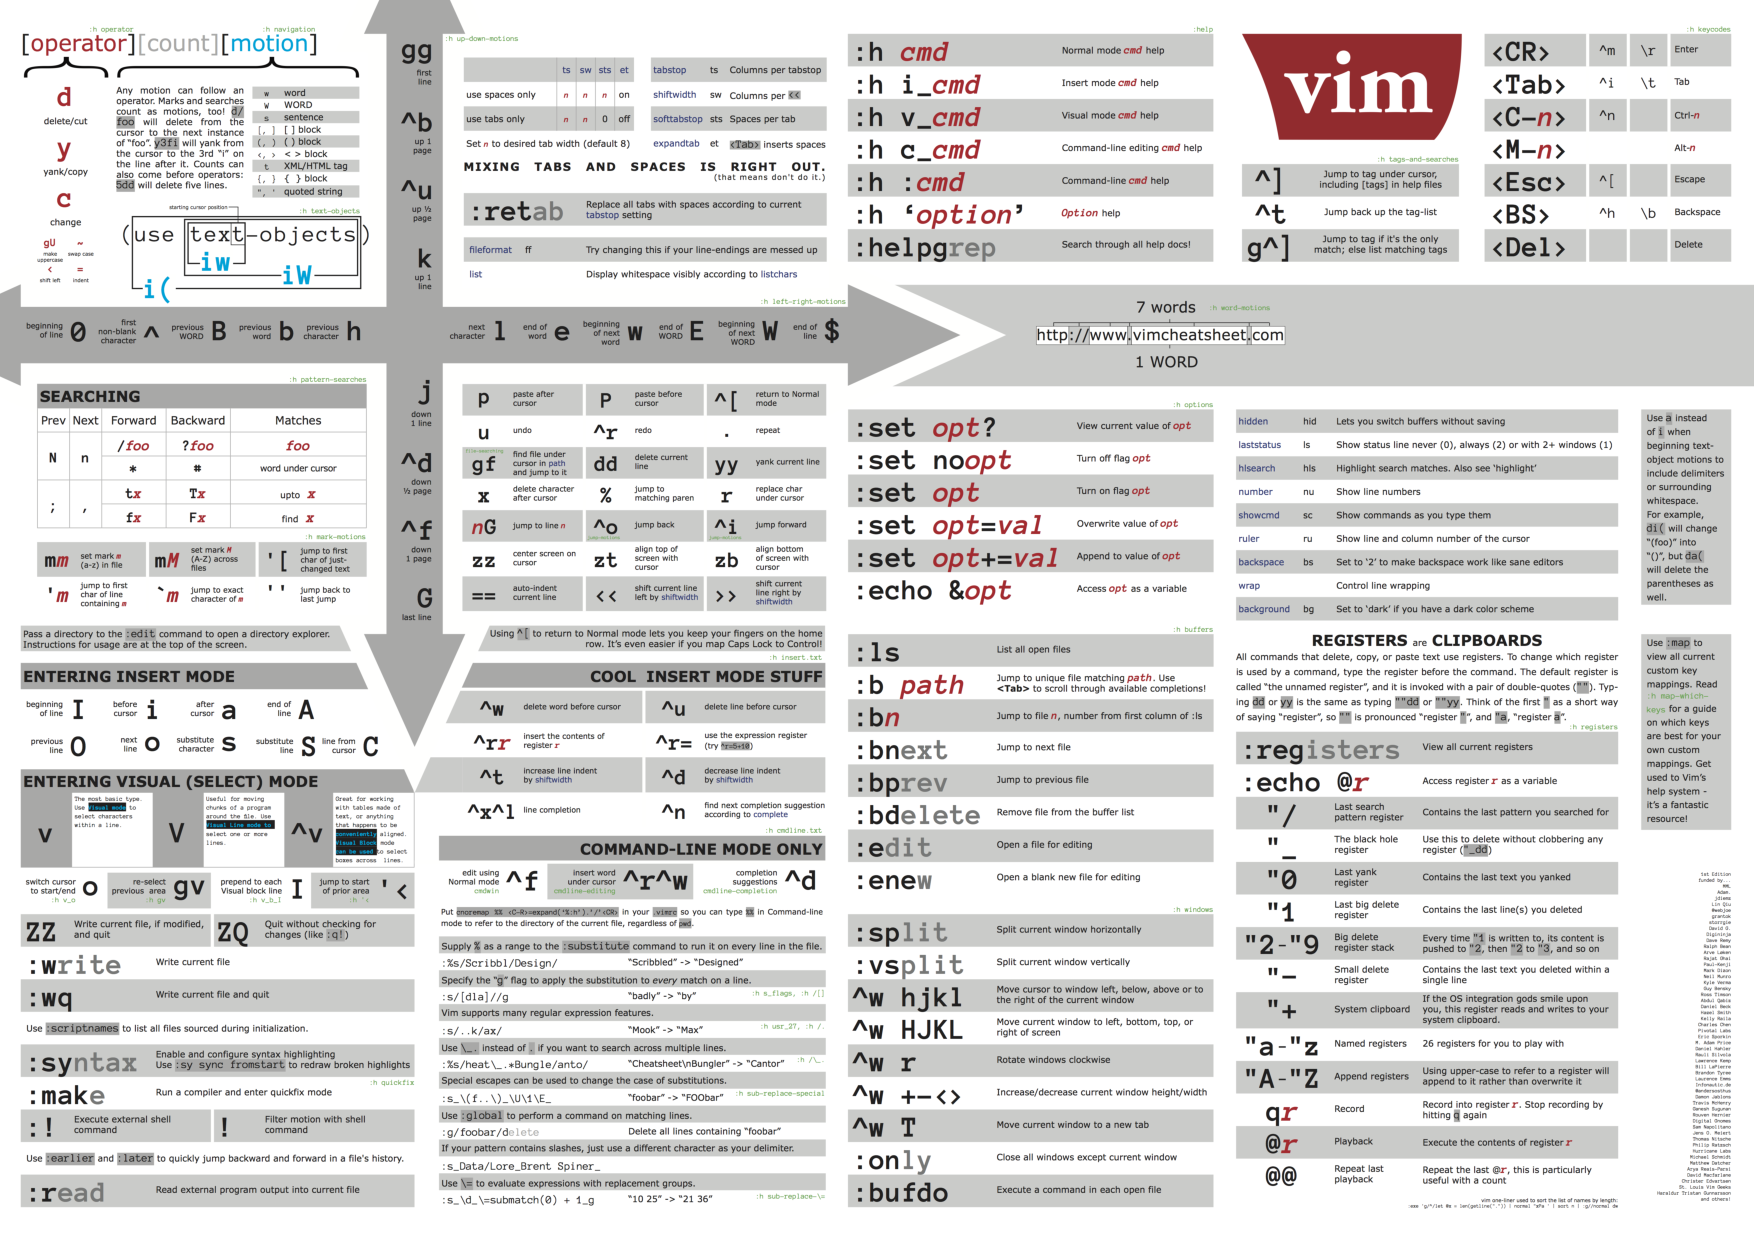
\includepdf{fig/vim.pdf}

\end{document}
